\section{Performance}

\figref{performanceNorm} shows the normalized score, number of hits in 90 seconds, for each of the display types and all participants. A similar figure with non-normalized values can be found in the appendix at page \textbf{TODO}. \textit{Delay} refers to the \textit{added} delay, which means that "No delay" translates to the inherent system delay of $250 ms$. The numerical values together with the standard deviation (SD) is reported in table \ref{score}. In addition, the percentage difference in means between displays is also reported in that table. The statistical significance and effect size between conditions can be seen in table \ref{score2}.

Using normalized scores, participants performed on average 20.29\% better using the predictive display versus no predictive display, $t(56)=4.82$, $p<.001$, $d=0.735$. In comparison, the subjects performed on average 153.32\% better in the no delay condition versus the delayed condition without predictive help, $t(56)=23.04$, $p<.001$, $d=4.413$. All differences are statistically significant.


\begin{figure}[h!]
    \centering
    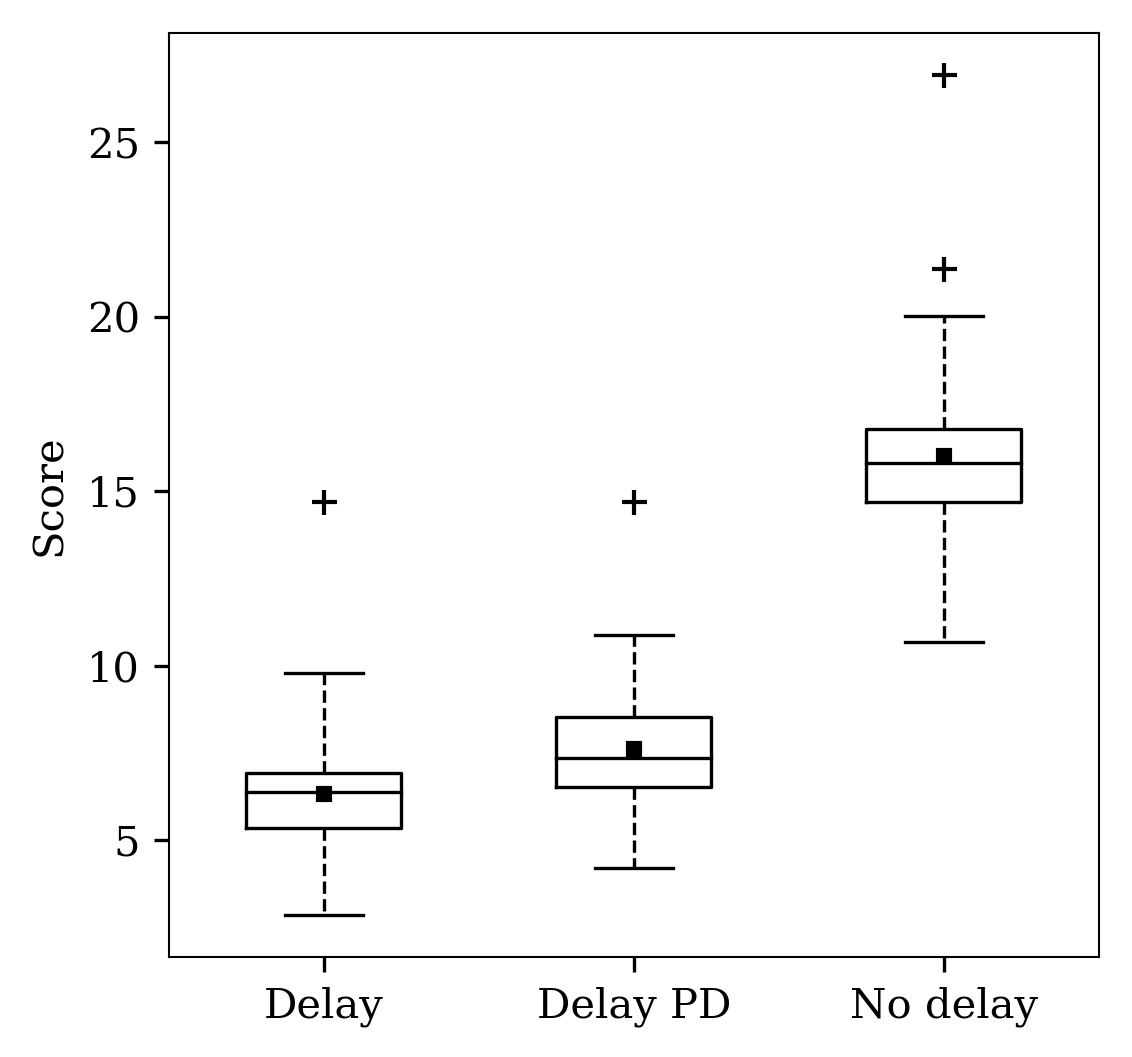
\includegraphics[scale=0.85]{performance_norm}
    \caption{Normalized score for each display type}
    \label{performanceNorm}
\end{figure}

% Please add the following required packages to your document preamble:
% \usepackage{booktabs}
\begin{table}[]
\small
\centering
\caption{Normalized mean scores and standard deviation (SD).}
\label{score}
\begin{tabularx}{\textwidth}{@{}XXXXX@{}}
\toprule
Differentiation & Group       & Display  & Score & SD \\ \midrule
None            & All N=57    & Delay    & 6.24  & 1.39               \\
                &             & Delay PD & 7.52  & 1.43               \\
                &             & No delay & 15.87 & 1.99               \\ \addlinespace
Gender          & Male n=38   & Delay    & 6.65  & 1.25               \\
                &             & Delay PD & 7.95  & 1.43               \\
                &             & No delay & 17.30 & 1.71               \\ \addlinespace
                & Female n=19 & Delay    & 5.39  & 1.49               \\
                &             & Delay PD & 6.61  & 1.35               \\
                &             & No delay & 13.10 & 2.17               \\ \addlinespace
Gaming          & Daily n=2   & Delay    & 7.92  & 0.37               \\
                &             & Delay PD & 10.21 & 1.40               \\
                &             & No delay & 18.36 & 1.77               \\ \addlinespace
                & Weekly n=15 & Delay    & 6.27  & 1.22               \\
                &             & Delay PD & 8.17  & 1.51               \\
                &             & No delay & 17.62 & 2.04               \\ \addlinespace
                & Monthly n=8 & Delay    & 7.05  & 1.32               \\
                &             & Delay PD & 7.77  & 0.64               \\
                &             & No delay & 17.68 & 0.95               \\ \addlinespace
                & Yearly n=17 & Delay    & 6.65  & 1.26               \\
                &             & Delay PD & 7.66  & 1.73               \\
                &             & No delay & 15.98 & 2.25               \\ \addlinespace
                & Never n=15  & Delay    & 5.06  & 1.46               \\
                &             & Delay PD & 6.21  & 1.16               \\
                &             & No delay & 12.73 & 1.79               \\ \bottomrule
\end{tabularx}
\end{table}
% Please add the following required packages to your document preamble:
% \usepackage{booktabs}
\begin{table}[]
\centering
\caption{Paired samples t-test and Cohen's d effect size}
\label{score2}
\begin{tabularx}{\textwidth}{@{}llYYYY@{}}
\toprule
\multicolumn{2}{c}{Pair} & \multicolumn{3}{c}{t-test for Equality of Means} &       \\ \cmidrule(lr){3-5}
\multicolumn{2}{l}{}     & t                  & df             & p                   & d     \\ \midrule
Delay       & Delay PD   & 4.82               & 56             & $<$.001             & 0.735 \\
Delay       & No delay   & 23.04              & 56             & $<$.001             & 4.413 \\
Delay PD    & No delay   & 19.52              & 56             & $<$.001             & 3.861 \\ \bottomrule
\end{tabularx}
\end{table}


\section{Task load index}

\figref{tlx} shows the reported NASA TLX scores. The height of the bar describes the mean value while the whiskers shows the SD. There are no big differences between condition one and two. The only significant differences between those two conditions can be found in the \emph{performance}, t(56)=3.24, p=0.002, d=0.360 and \emph{frustration}, t(56)=2.15, p=0.036, d=0.271 metric. This means that the subjects felt less frustration and evaluated their performance as better when using the predictive display.


\begin{figure}[h!]
    \centering
    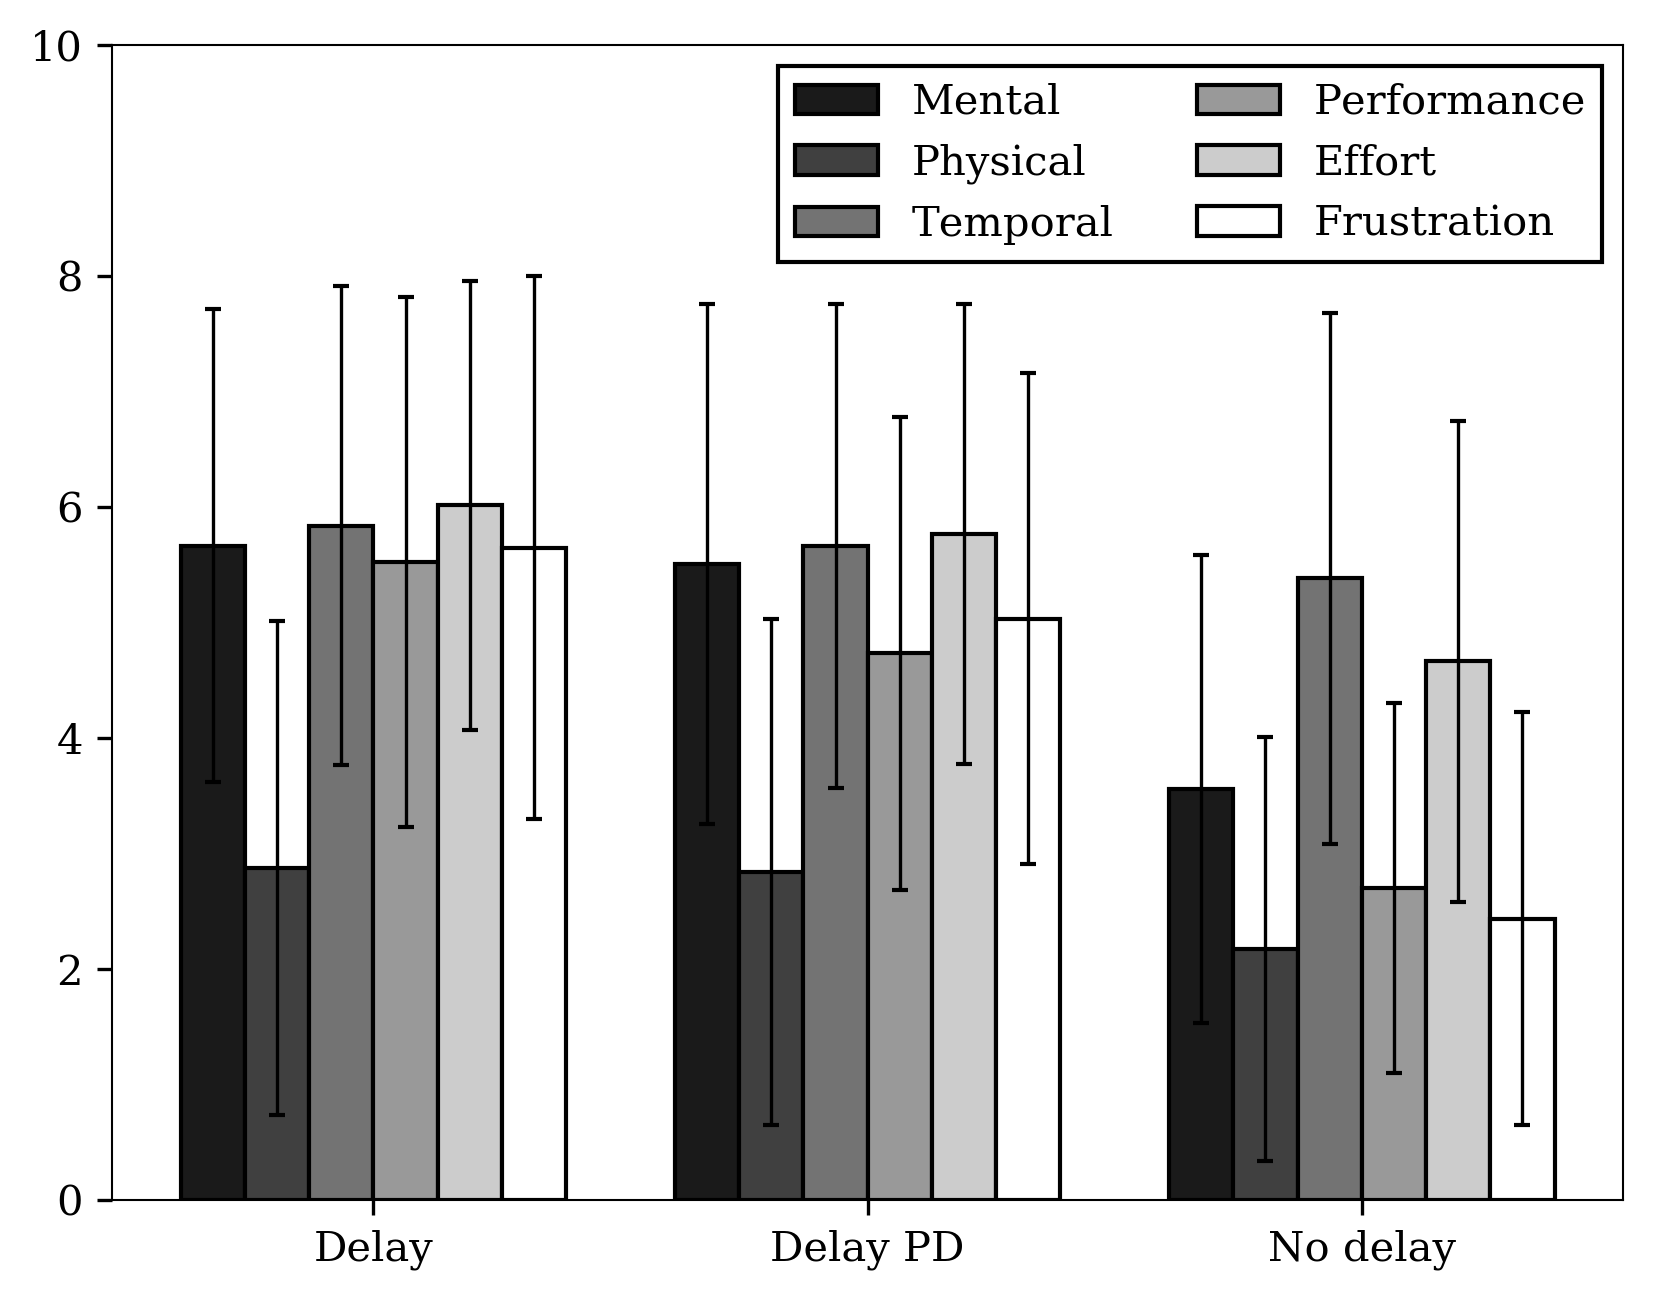
\includegraphics[scale=0.85]{nasa_tlx_bar}
    \caption{NASA TLX (task load index) results for each display type. Lower is better.}
    \label{tlx}
\end{figure}